\subsection{Vggface2}
Due to its broad scope and comprehensive coverage, VGGFace2 represents a significant leap in the field of facial recognition. It responds to the demand for a large dataset that can be used to train deep convolutional neural networks (CNNs) to accurately identify faces across a range of identities and demographics. VGGFace2 delivers a robust and wide set of facial data for training and assessing face recognition models, with over 3.3 million photos of more than 9,000 different people.

Each image in the collection has accurate and consistent information because of the rigorous annotation and labeling. The bounding box coordinates, which identify the face's placement inside the picture, are included in the annotations. This enables practitioners and academics to train and test face recognition algorithms that are purely concerned with the facial region.


\begin{figure}[h]
    \centering
    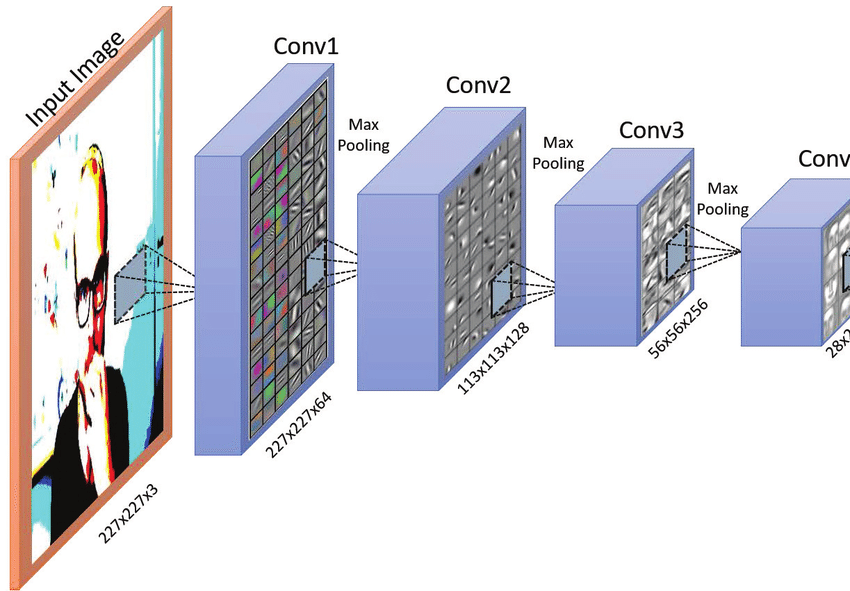
\includegraphics[width= 5in ]{img/The-VGG-Face-architecture-visualizing-low-to-high-level-features-captured-as-a-facial.png}
    \caption{Vggface2 Architecture}
\end{figure}